\begin{singlespacing}
\chapter{Searches in ATLAS}
\label{chapter:searches}
%
\begin{epigraphs}
\qitem{%
One way is to make it so simple that there are \emph{obviously} no deficiencies
and the other way is to make it so complicated that there are no \emph{obvious}
deficiencies.%
}%
{Tony~Hoare,
\textit{The Emperor’s Old Clothes},
1981~\cite{hoare2007emperor}}
\end{epigraphs}
\end{singlespacing}

Our task in scientific data analysis is to distil an informative
message from data and to report that message to the wider community.
From any given data there are many possible messages that could be extracted,
and those messages will have different values to different recipients of our
messages --- our data analysis is not an automatic process, but a result
of many judgements that are informed by theory, convention, and intuition.

To clarify our later description of the $\twoljets$ search in
Chapter~\ref{chapter:2ljets}, this chapter introduces the basic theory and
practice of data analysis and its manifestations in the \atlas\ SUSY community.

Theoretical data analysis in the tightly coupled fields of probability theory
and decision theory is introduced in Section~\ref{sec:searces_data_analysis}.
An attempted alternative formulation, frequentist theory, is discussed in
Section~\ref{sec:searches_frequentist} for its relevance to our methods.
Standard practice in this field of research does not strictly follow
frequentist methods, but patches up some of their pathologies with modified
approaches that we describe in Section~\ref{sec:searches_practice}.
Searches for Supersymmetric signals in \atlas\ follow a standard strategy for
their data analysis; its procedures, nomenclature, and parametric modelling
are introduced in Section~\ref{sec:searches_searches}.


\section{Data analysis}
\label{sec:searces_data_analysis}
How many jelly beans are in the jar of Figure~\ref{fig:significant_beans}?
Your answer depends not only on what you observe from the figure, but also on
what else you know about cartoon jars of beans, and on what reward is on offer.
Each answer is a decision that depends both on what the possible rewards are,
and on which numbers of beans you subjectively infer to be likely.
We shall return to this example after developing some probability and decision
theory.

\begin{figure}[tp]
\centering
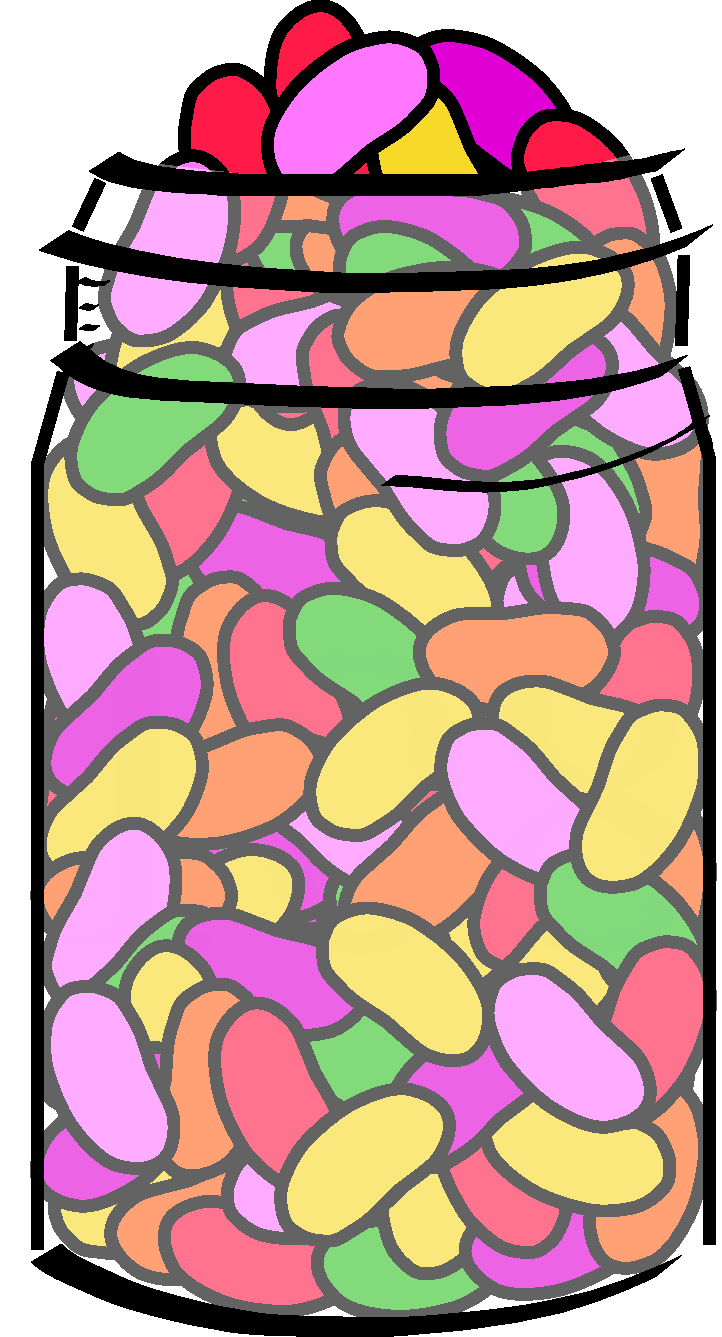
\includegraphics[width=0.25\textwidth]{figures/searches_beans.pdf}
\caption[
How many beans are in the jar?
]{%
How many beans are in the jar? This jar of jelly beans is a vehicle for our
discussion of inference and decision theory.
Please write your guess on this page.
The first correct answer wins a gold star.
}
\label{fig:significant_beans}
\end{figure}

We begin with what probability is.
At its most abstract, a probability a proportion of stuff within a larger
whole, and probabilities are useful because they can be manipulated with an
algebra that corresponds to how one naturally manipulates such proportions.

\paragraph{Probability, abstract}
A probability $\prob{b}{a}$ is a number that quantifies the proportion
of $b$ within $a$, and can be expressed as a ratio of measures
as~\cite{axioms1010038}
\begin{equation}
\label{eqn:searches_prob_ratio}
\prob{b}{a} = \frac{m(b, a)}{m(a)},
\end{equation}
in which $m(x)$ is a measure (a non-negative quantity assigned to its
argument, such as mass of tea in a cup), and the comma ``,'' means `and'
(logical and or set intersection or any other equivalent operation).
To continue that example, $\prob{b}{a}$ could be a proportion of tea within
a spoon within a cup, where $m(b \land a)$ measures the volume of tea in a
teaspoon that is partially submerged in the cup.%
\footnote{%
All probabilities are conditional in this definition; $\probc{b}$ alone does
not exist unless the conditioning information $a$ is implicit from context.%
}

Logic is an important application of probability for which $a$ and $b$ are
interpreted as logical propositions, and
$\prob{b}{a}$ is the degree to which $a$ implies $b$, with the limiting cases
that $\prob{b}{a} = 1$ when $a$ implies $b$ and $\prob{b}{a} = 0$ when $a$
disproves $b$.
Indeed Cox's theorem derives the laws of probability by requiring compatibility
with Boolean logic~\cite{
cox1946probability,
cox1961algebra,
garrett1998nand,
jaynes2003probability
keynes1920treatise,
}.
Probability works for logic and it works \emph{for tea, too}.

Probability algebra has two rules that can derive from the measure ratio of
Equation~\ref{eqn:searches_prob_ratio}:
a \textbf{product rule}
\begin{equation}
\prob{c, b}{a} = \prob{c}{b, a}\times \prob{b}{a},
\end{equation}
and a \textbf{sum rule}
\begin{equation}
\prob{c\textrm{ or }b}{a} = \prob{c}{a} + \prob{b}{a} - \prob{c, b}{a}.
\end{equation}
To avoid of this subtraction we prefer split any problem into orthogonal or
disjoint states; for such cases, the normalization condition is that
\begin{equation}
\sum_i \prob{b_i}{a} = 1.
\end{equation}
These rules are basic and well known, but we state them here to support the
following statements of how probabilities can be applied for practical
results.%
\footnote{%
The formulation with sums and products is not strictly unique, but all
alternatives are equivalent up to an invertible
transformation~\cite{axioms1010038}.
This choice is usually best because it uses ordinary addition and
multiplication.
In numerical analysis, however, it is often practical to use $\log$
probabilities (to avoid overflows outside the range representable by floating
point numbers(, thus changing multiplication to addition, and addition to
the `$\log$-add-$\exp$' operation.
}

\paragraph{Probability, applied}
% science snake

Probabilistic data analysis proceeds as follows:
\begin{enumerate}
\item Predict new data $d$ with probability $\prob{d}{\ldots}$.
\item Update your predictions with the observed data to $\prob{x}{d, \ldots}$.
\item Go to 1.
\end{enumerate}

% evidence

% bayes
Bayes' theorem is an infamous and necessary result of probability.

% posterior

\paragraph{Probability assignments}
infamously arbitrary and subjective. This is reality. They are.
Consider this simple mathematical example with two propositions
$a=\textrm{``}x\textrm{ is even''}$ and
$b=\textrm{``}x\textrm{ equals }2\textrm{''}$.
Clearly $\prob{a}{b} = 1$ since $2$ is indeed even.
But what is $\prob{b}{a}$? We don't know. Perhaps one could argue symmetry
across all even numbers, but there are infinitely many of them so that
probability distribution could not be normalized.

\TODO{\ldots}


\paragraph{Decision theory}


% summary

Figure~\ref{fig:searches_baton_roue_bayes}

\begin{figure}[tp]
\centering

\includegraphics[width=0.65\textwidth]{figures/searches_baton_roue_bayes.jpg}
\caption[
Bayesian analysis produces two outputs: the evidence and posterior
]{%
Bayesian analysis produces two outputs: the
evidence $\prob{d}{h}$ and
posterior $\prob{x}{d,h}$ for hypothesis $h$, data $d$, and parameters $x$.
Posterior-only, semi-Bayesian methods are legitimately criticized because they
do not challenge the hypotheses that assign their priors $\prob{x}{h}$.
Since the evidence is a likelihood function over hypotheses, considering the
evidence can challenge those priors.
\\[0.5em]
Cartoon adapted from ``Baton roue'' by
Corentin~Penloup~\cite{penloup2011baton}.
}
\label{fig:searches_baton_roue_bayes}
\end{figure}


\begin{singlespacing}
\section{Frequentist theory}
\label{sec:searches_frequentist}
\begin{epigraphs}
\qitem{%
Within this theory, statistical methods of great practical usefulness have been
developed, and its statements can and frequently do contribute in a vague way
to the interpretation of data. \ldots%
}%
{John~W.~Pratt,
\textit{Review: Testing Statistical Hypotheses},
1961~\cite{pratt1961testing}}
\end{epigraphs}
\end{singlespacing}

Figure~\ref{fig:searches_significant}

\begin{figure}[tp]
\centering
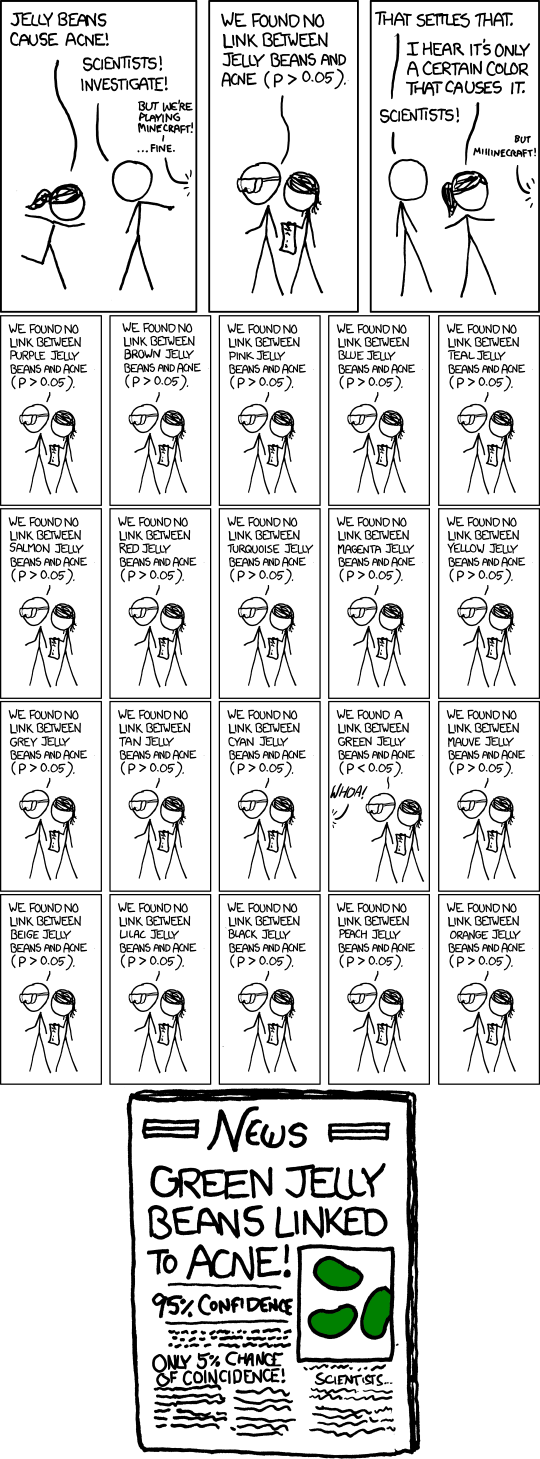
\includegraphics[width=0.55\textwidth]{figures/searches_significant_shrink.png}
\\
\begin{footnotesize}
`So, uh, we did the green study again and got no link. It was probably a{-}{-}'
\\
`RESEARCH CONFLICTED ON GREEN JELLY BEAN ACNE LINK; MORE~STUDY~RECOMMENDED!'
\end{footnotesize}
\caption[
``Significant'' by Randall~Munroe
]{%
``Significant'' by Randall~Munroe~\cite{xkcd2011significant}.
}
\label{fig:searches_significant}
\end{figure}


\begin{singlespacing}
\section{Post-frequentist practice}
\label{sec:searches_practice}
\begin{epigraphs}
\qitem{%
\ldots\ But this book, by its very excellence, its thoroughness, lucidity and
precision, intensifies my growing feeling that nevertheless the theory is
arbitrary, be it however ``objective,'' and the problems it solves, however
precisely it may solve them, are not even simplified theoretical counterparts
of the real problems to which it is applied.%
}%
{John~W.~Pratt,
\textit{Review: Testing Statistical Hypotheses},
1961~\cite{pratt1961testing}}
\end{epigraphs}
\end{singlespacing}


% significance measures
The ATLAS-recommended significance measure~\cite{atlas_significance} is
\begin{align}
\label{eqn:significance_atlas}
S_\mathrm{\atlas}(n; \mu, \sigma) =~&
\sqrt{2} \times
\mathrm{sign}(n - \mu) \times
\\[0.2em] \nonumber
&
\sqrt{
n\log\left(\frac{n(\mu + \sigma^2)}{\mu^2 + n\sigma^2}\right)
- \frac{\mu^2}{\sigma^2}\log\left(
1 + \frac{\sigma^2(n - \mu)}{\mu(\mu + \sigma^2)}
\right)
}
,
\end{align}
in an appropriate limit where $0\log(0x) = 0$ for the $n=0$ case.


\section{Searches}
\label{sec:searches_searches}
% histograms, CR VR SR, systematics
% histfactory

To model the consequences of these many factors of uncertainty, each factor is
assigned a real-valued parameter which when varied changed the expected yields
in the hisogram bins of the search.
In this way, we form a statistical model which is a function
\begin{equation}
H_{\!f}(\vec \theta) \rightarrow (\vec \mu, \log f)
\end{equation}
from the parameters $\theta$ to Poisson expectations $\vec\mu$ the histogram
bins and a regularization term $\log f$ which is maximized in fitting.

\histfactory~\cite{cranmer2012histfactory}
\pyhf~\cite{heinrich2021pyhf}
\histfitter~\cite{Besjes_2015,baak2015histfitter}


\clearpage

Hello again
